\documentclass{article}
\usepackage[utf8]{inputenc}

\title{PS7 Li}
\author{Donald Li }
\date{March 2018}

\usepackage{natbib}
\usepackage{graphicx}

\begin{document}

\maketitle

\section{Part 6}
After looking through the data set it seems to be MNAR. Some people may not feel comfortable in revealing their incomes. Between characteristics and missingness there are 560 missing obs out of 2246. 

\section{Part 7}
The imputation methods will never be the exact beta value of .093. However, with each level of imputation we get a little bit closer. Casewise deletion gives the worst, followed by Mean then finally Predictive mean matching gives us the best. 


\section{Part 8}
For my final project we are using twitter data for sentiment analysis! I have already worked on a practice data set of fake/real text messages to cut my teeth at natural language processing! I am very excited to see the results. Right now we are in the gather data phase. 

\begin{table}[!htbp] \centering 
  \caption{} 
  \label{} 
\begin{tabular}{@{\extracolsep{5pt}}lccccc} 
\\[-1.8ex]\hline 
\hline \\[-1.8ex] 
Statistic & \multicolumn{1}{c}{N} & \multicolumn{1}{c}{Mean} & \multicolumn{1}{c}{St. Dev.} & \multicolumn{1}{c}{Min} & \multicolumn{1}{c}{Max} \\ 
\hline \\[-1.8ex] 
logwage & 1,669 & 1.625 & 0.386 & 0.005 & 2.261 \\ 
hgc & 1,669 & 12.556 & 2.322 & 0 & 18 \\ 
tenure & 1,669 & 5.225 & 5.095 & 0.000 & 24.750 \\ 
age & 1,669 & 39.171 & 3.085 & 34 & 45 \\ 
\hline \\[-1.8ex] 
\end{tabular} 
\end{table} 

\begin{table}[!htbp] \centering 
  \caption{} 
  \label{} 
\begin{tabular}{@{\extracolsep{5pt}}lc} 
\\[-1.8ex]\hline 
\hline \\[-1.8ex] 
 & \multicolumn{1}{c}{\textit{Dependent variable:}} \\ 
\cline{2-2} 
\\[-1.8ex] & logwage \\ 
\hline \\[-1.8ex] 
 hgc & 0.062$^{***}$ \\ 
  & (0.005) \\ 
  & \\ 
 collegenot college grad & 0.146$^{***}$ \\ 
  & (0.035) \\ 
  & \\ 
 tenure & 0.023$^{***}$ \\ 
  & (0.002) \\ 
  & \\ 
 age & $-$0.001 \\ 
  & (0.003) \\ 
  & \\ 
 marriedsingle & $-$0.024 \\ 
  & (0.018) \\ 
  & \\ 
 Constant & 0.639$^{***}$ \\ 
  & (0.146) \\ 
  & \\ 
\hline \\[-1.8ex] 
Observations & 1,669 \\ 
R$^{2}$ & 0.195 \\ 
Adjusted R$^{2}$ & 0.192 \\ 
Residual Std. Error & 0.346 (df = 1663) \\ 
F Statistic & 80.508$^{***}$ (df = 5; 1663) \\ 
\hline 
\hline \\[-1.8ex] 
\textit{Note:}  & \multicolumn{1}{r}{$^{*}$p$<$0.1; $^{**}$p$<$0.05; $^{***}$p$<$0.01} \\ 
\end{tabular} 
\end{table} 

\begin{table}[!htbp] \centering 
  \caption{} 
  \label{} 
\begin{tabular}{@{\extracolsep{5pt}}lc} 
\\[-1.8ex]\hline 
\hline \\[-1.8ex] 
 & \multicolumn{1}{c}{\textit{Dependent variable:}} \\ 
\cline{2-2} 
\\[-1.8ex] & logwage \\ 
\hline \\[-1.8ex] 
 hgc & 0.062$^{***}$ \\ 
  & (0.005) \\ 
  & \\ 
 collegenot college grad & 0.146$^{***}$ \\ 
  & (0.035) \\ 
  & \\ 
 tenure & 0.023$^{***}$ \\ 
  & (0.002) \\ 
  & \\ 
 age & $-$0.001 \\ 
  & (0.003) \\ 
  & \\ 
 marriedsingle & $-$0.024 \\ 
  & (0.018) \\ 
  & \\ 
 Constant & 0.639$^{***}$ \\ 
  & (0.146) \\ 
  & \\ 
\hline \\[-1.8ex] 
Observations & 1,669 \\ 
R$^{2}$ & 0.195 \\ 
Adjusted R$^{2}$ & 0.192 \\ 
Residual Std. Error & 0.346 (df = 1663) \\ 
F Statistic & 80.508$^{***}$ (df = 5; 1663) \\ 
\hline 
\hline \\[-1.8ex] 
\textit{Note:}  & \multicolumn{1}{r}{$^{*}$p$<$0.1; $^{**}$p$<$0.05; $^{***}$p$<$0.01} \\ 
\end{tabular} 
\end{table} 

\begin{figure}[h!]
\centering
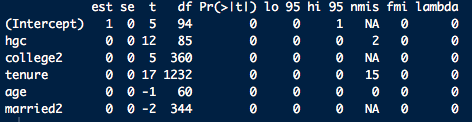
\includegraphics[scale=1]{MiceImp_table.png}
\caption{Mice_Imp}
\end{figure}
\end{document}
